\documentclass[11pt]{article}
\usepackage[letterpaper,landscape,margin=1.5cm]{geometry}
\usepackage{enumitem}
\usepackage{xcolor}
\usepackage{microtype}
\usepackage{tikz}
\usetikzlibrary{positioning,calc}
\usepackage[hidelinks]{hyperref}

\setlist{nosep, leftmargin=1.4em}
\setlength{\parindent}{0pt}
\setlength{\parskip}{0.3em}
\pagestyle{empty}

\newcommand{\code}[1]{\texttt{#1}}

\definecolor{v5}{RGB}{200,30,30}
\definecolor{sda}{RGB}{30,90,200}
\definecolor{scl}{RGB}{200,170,0}
\definecolor{vcc}{RGB}{225,115,0}
\definecolor{dpm}{RGB}{120,120,120}
\definecolor{uart}{RGB}{200,25,180}
\definecolor{swd}{RGB}{110,50,200}

\tikzset{
  blk/.style={draw, rounded corners=2pt, minimum height=9mm, minimum width=14mm, align=center, font=\small, fill=white},
  bo/.style={draw, very thick, fill=green!8, minimum width=30mm, minimum height=26mm},
  ina/.style={draw, very thick, fill=gray!15, minimum width=34mm, minimum height=16mm, align=center, font=\small},
  pin/.style={font=\scriptsize\ttfamily, inner sep=1pt},
  w5/.style={very thick, v5},
  wdp/.style={thick, dpm},
  wsda/.style={thick, sda},
  wscl/.style={thick, scl},
  wv/.style={thick, vcc},
  wg/.style={thick, black},
  wu/.style={thick, uart},
  ws/.style={thick, swd},
  wd/.style={thick, gray, densely dashed},
  lbl/.style={font=\scriptsize, text=black!75, align=center},
  dot/.style={circle, fill, inner sep=1.1pt},
}

\begin{document}

{\Large\bfseries H723 power measurement --- how to connect it}\hfill{\small 2 November 2026, revision 2}

\smallskip
{\small One module, \textbf{M1} (\code{R100}, address \code{0x40}), in the 5\,V wire between the laptop and the H723, read by
the spare F411, which is also the USB breakout. \textbf{Nothing is cut, nothing is bought, every cable is a standard USB
cable.}}

\smallskip
\noindent\fbox{\parbox{0.985\linewidth}{\small\textbf{All already on the bench:} the \textbf{spare F411} running the logger
firmware (its own USB never switched on; its USB-C socket wired to its header pins \code{5V}, \code{G}, \code{A11}, \code{A12},
so it is the USB-C breakout and the logger at once), one of your USB-A \textbf{female} breakouts, M1, the debugger and
jumper wires. Pictures: \code{power-wiring-h723-3d.pdf}.}}

\begin{center}
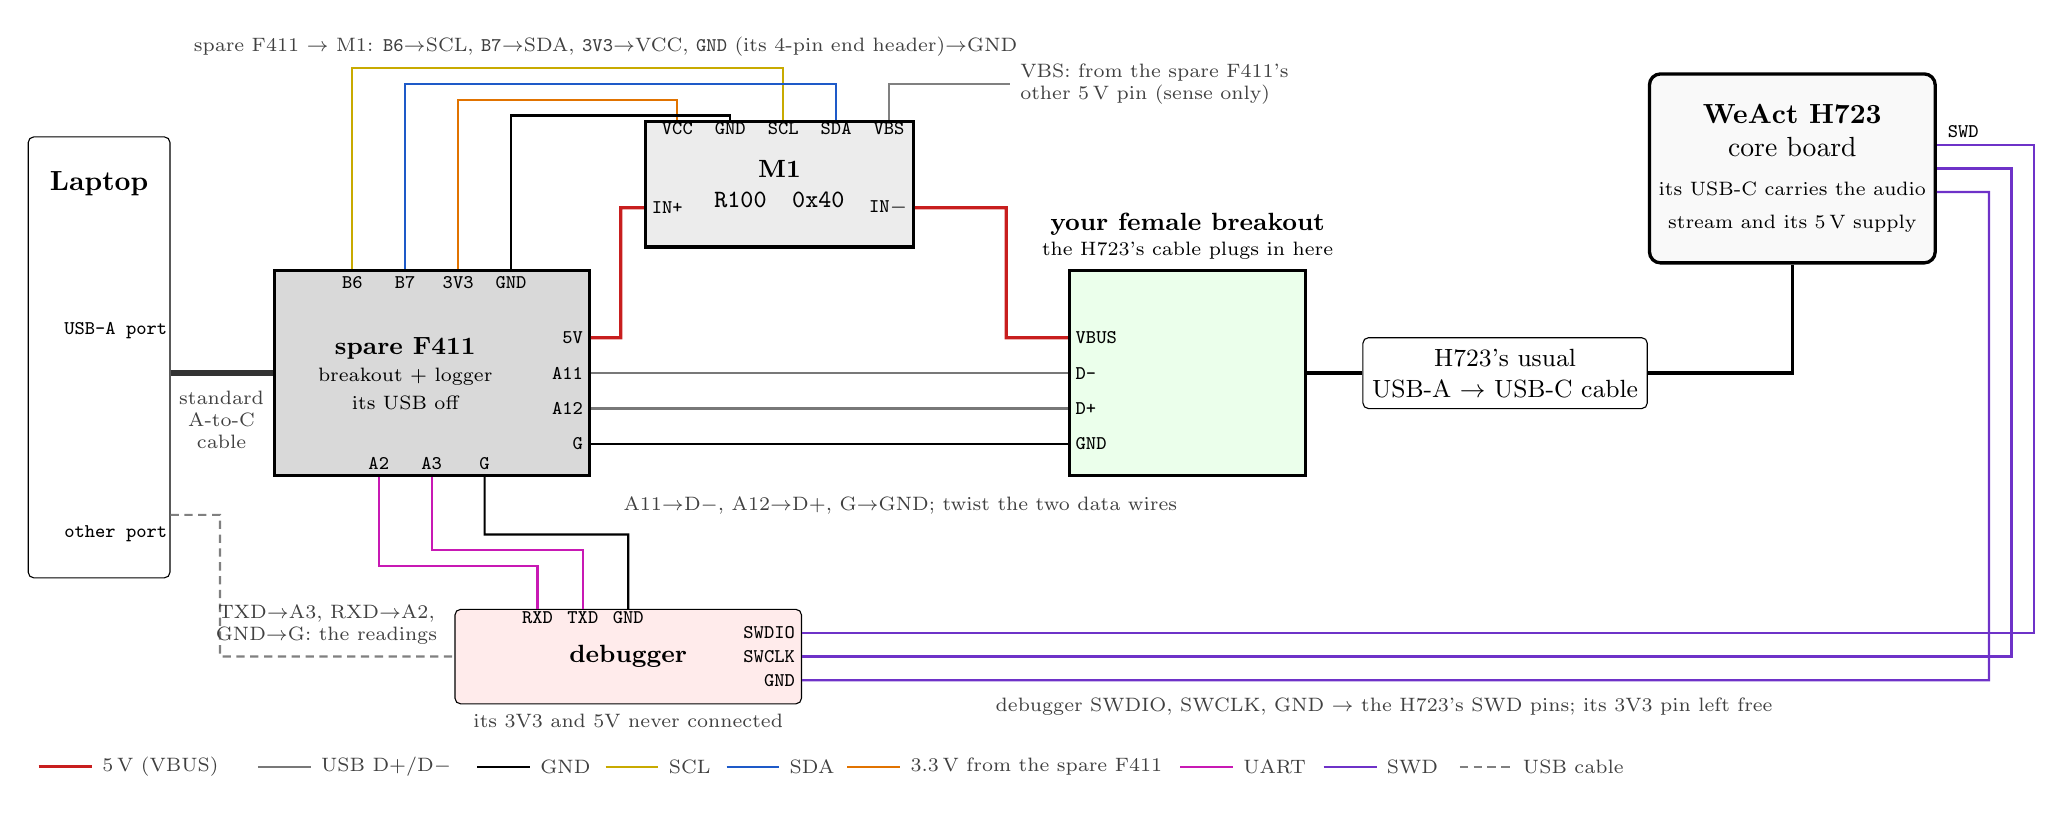
\begin{tikzpicture}[x=0.96cm,y=1cm]

%---------- laptop ----------
\node[blk, minimum width=18mm, minimum height=56mm] (lap) at (0,0.2) {};
\node[font=\bfseries] at (0,2.4) {Laptop};
\coordinate (pA) at ($(lap.east)+(0,-0.2)$);   % y = 0
\coordinate (pD) at ($(lap.east)+(0,-2.0)$);   % y = -1.8
\node[pin, anchor=south east] at ($(pA)+(0,0.4)$) {USB-A port};
\node[pin, anchor=north east] at ($(pD)+(0,-0.1)$) {other port};

%---------- the spare F411 (pins: east = to the breakout, north = to M1, south = to the debugger) ----------
\node[bo, fill=gray!30, minimum width=40mm] (mb) at (4.4,0) {};
\draw[line width=2.4pt, black!80] (pA) -- (mb.west);
\node[lbl, anchor=north] at ($(pA)!0.5!(mb.west)+(0,-0.1)$) {standard\\A-to-C\\cable};
\node[font=\small, align=center] at ($(mb.center)+(-0.35,0)$) {\textbf{spare F411}\\[-1pt]{\scriptsize breakout + logger}\\[-1pt]{\scriptsize its USB off}};
\foreach \p/\y/\t in {VBUS/0.45/5V,D-/0.0/A11,D+/-0.45/A12,GND/-0.9/G}{
  \coordinate (m\p) at ($(mb.east)+(0,\y)$);
  \node[pin, anchor=east, fill=gray!30] at ($(m\p)+(-0.06,0)$) {\t};}
\foreach \p/\x in {B6/-1.05,B7/-0.35,3V3/0.35,GNDs/1.05}{
  \coordinate (n\p) at ($(mb.north)+(\x,0)$);}
\foreach \p/\x/\t in {B6/-1.05/B6,B7/-0.35/B7,3V3/0.35/3V3,GNDs/1.05/GND}{
  \node[pin, anchor=north, fill=gray!30] at ($(mb.north)+(\x,-0.05)$) {\t};}
\foreach \p/\x/\t in {A2/-0.7/A2,A3/0.0/A3,G2/0.7/G}{
  \coordinate (s\p) at ($(mb.south)+(\x,0)$);
  \node[pin, anchor=south, fill=gray!30] at ($(s\p)+(0,0.05)$) {\t};}

%---------- female breakout (pins on its left) ----------
\node[bo] (fb) at (14.4,0) {};
\node[font=\small, anchor=south, align=center] at (fb.north) {\textbf{your female breakout}\\[-2pt]{\scriptsize the H723's cable plugs in here}};
\foreach \p/\y in {VBUS/0.45,D-/0.0,D+/-0.45,GND/-0.9}{
  \coordinate (f\p) at ($(fb.west)+(0,\y)$);
  \node[pin, anchor=west] at ($(f\p)+(0.06,0)$) {\p};}

%---------- straight across ----------
\draw[wdp] (mD-) -- (fD-);
\draw[wdp] (mD+) -- (fD+);
\draw[wg]  (mGND) -- (fGND);
\node[lbl, anchor=north] at (10.6,-1.45) {A11$\to$D$-$, A12$\to$D+, G$\to$GND; twist the two data wires};

%---------- M1 in VBUS ----------
\node[ina] (m1) at (9.0,2.4) {\bfseries M1\\\code{R100}\quad\code{0x40}};
\node[pin, anchor=west] at ($(m1.west)+(0.06,-0.3)$) {IN+};
\node[pin, anchor=east] at ($(m1.east)+(-0.06,-0.3)$) {IN$-$};
\draw[w5] (mVBUS) -- (6.9,0.45) -- (6.9,2.1) -- ($(m1.west)+(0,-0.3)$);
\draw[w5] ($(m1.east)+(0,-0.3)$) -- (12.0,2.1) -- (12.0,0.45) -- (fVBUS);
% M1 top pins: VCC GND SCL SDA, and VBUS (sense) on the right
\foreach \p/\x in {VCC/-1.35,GND/-0.65,SCL/0.05,SDA/0.75}{
  \coordinate (t\p) at ($(m1.north)+(\x,0)$);
  \node[pin, anchor=north] at (t\p) {\p};}
\coordinate (tVB) at ($(m1.north)+(1.45,0)$);
\node[pin, anchor=north] at (tVB) {VBS};
\draw[thick, gray] (tVB) -- ++(0,0.45) -- ++(1.6,0) node[lbl, right, text=black!75, align=left] {VBS: from the spare F411's\\other 5\,V pin (sense only)};

%---------- spare F411 -> M1 over I2C ----------
\draw[wscl] (nB6) -- ++(0,2.55) -| (tSCL);
\draw[wsda] (nB7) -- ++(0,2.35) -| (tSDA);
\draw[wv]   (n3V3) -- ++(0,2.15) -| (tVCC);
\draw[wg]   (nGNDs) -- ++(0,1.95) -| (tGND);
\node[lbl, anchor=south] at (6.7,3.9) {spare F411 $\to$ M1: \code{B6}$\to$SCL, \code{B7}$\to$SDA, \code{3V3}$\to$VCC,
\code{GND} (its 4-pin end header)$\to$GND};

%---------- debugger ----------
\node[blk, minimum width=44mm, minimum height=12mm, fill=red!8] (dbg) at (7.0,-3.6) {\bfseries debugger};
\node[lbl, anchor=north] at (dbg.south) {its 3V3 and 5V never connected};
\draw[wd] (pD) -- (1.6,-1.8) |- (dbg.west);
\foreach \p/\x/\t in {RXD/-1.2/RXD,TXD/-0.6/TXD,GNDu/0.0/GND}{
  \coordinate (d\p) at ($(dbg.north)+(\x,0)$);
  \node[pin, anchor=north] at (d\p) {\t};}
\draw[wu] (dRXD) |- (3.7,-2.45) -- (sA2);
\draw[wu] (dTXD) |- (4.4,-2.25) -- (sA3);
\draw[wg] (dGNDu) |- (5.1,-2.05) -- (sG2);
\node[lbl, anchor=east] at (4.6,-3.2) {TXD$\to$A3, RXD$\to$A2,\\GND$\to$G: the readings};
\foreach \p/\y/\t in {DIO/0.3/SWDIO,CLK/0.0/SWCLK,GNDs/-0.3/GND}{
  \coordinate (e\p) at ($(dbg.east)+(0,\y)$);
  \node[pin, anchor=east] at ($(e\p)+(-0.05,0)$) {\t};}

%---------- cable and board ----------
\node[blk, minimum width=22mm] (cab) at (18.6,0) {H723's usual\\USB-A $\to$ USB-C cable};
\draw[very thick] (fb.east) -- (cab.west);
\node[draw, very thick, rounded corners=4pt, fill=gray!5, minimum width=36mm, minimum height=24mm, align=center] (h7) at (22.4,2.6) {\bfseries WeAct H723\\core board\\[2pt]{\scriptsize its USB-C carries the audio}\\{\scriptsize stream and its 5\,V supply}};
\draw[very thick] (cab.east) -| (h7.south);
\foreach \p/\y/\o in {DIO/0.3/25.6,CLK/0.0/25.3,GNDs/-0.3/25.0}{
  \coordinate (h\p) at ($(h7.east)+(0,\y)$);
  \draw[ws] (e\p) -- (\o,{-3.6+\y}) |- (h\p);}
\node[pin, anchor=south west] at ($(h7.east)+(0.1,0.35)$) {SWD};
\node[lbl, anchor=north] at (17.0,-4.0) {debugger SWDIO, SWCLK, GND $\to$ the H723's SWD pins; its 3V3 pin left free};

%---------- legend ----------
\begin{scope}[shift={(-0.8,-5.0)}]
\draw[w5] (0,0) -- ++(0.7,0) node[right, lbl] {5\,V (VBUS)};
\draw[wdp] (2.9,0) -- ++(0.7,0) node[right, lbl] {USB D+/D$-$};
\draw[wg] (5.8,0) -- ++(0.7,0) node[right, lbl] {GND};
\draw[wscl] (7.5,0) -- ++(0.7,0) node[right, lbl] {SCL};
\draw[wsda] (9.1,0) -- ++(0.7,0) node[right, lbl] {SDA};
\draw[wv] (10.7,0) -- ++(0.7,0) node[right, lbl] {3.3\,V from the spare F411};
\draw[wu] (15.1,0) -- ++(0.7,0) node[right, lbl] {UART};
\draw[ws] (17.0,0) -- ++(0.7,0) node[right, lbl] {SWD};
\draw[wd] (18.8,0) -- ++(0.7,0) node[right, lbl] {USB cable};
\end{scope}
\end{tikzpicture}
\end{center}

\vspace{-1.2em}
{\small
\begin{minipage}[t]{0.48\linewidth}
\textbf{Wire it, once} (the same for all three microcontroller boards)
\begin{enumerate}
\item Spare F411 \code{5V} $\to$ M1 \code{IN+}; M1 \code{IN-} $\to$ breakout VBUS (both are header pins on M1);
the spare F411's other \code{5V} $\to$ M1 \code{VBS}.
\item \code{A11} $\to$ D$-$, \code{A12} $\to$ D+, \code{G} $\to$ GND, spare F411 to the breakout.
\item \code{B6} $\to$ SCL, \code{B7} $\to$ SDA, \code{3V3} $\to$ VCC, \code{GND} $\to$ GND, spare F411 to M1.
\item Debugger \code{TXD} $\to$ \code{A3}, \code{RXD} $\to$ \code{A2}, \code{GND} $\to$ \code{G}; never its \code{3V3} or
\code{5V}.
\item With only the spare F411 plugged in and running the logger, \code{dmesg -w} prints nothing; its \code{5V} pin reads
about 4.7\,V; the readings arrive on the debugger's serial port.
\end{enumerate}
\end{minipage}\hfill
\begin{minipage}[t]{0.49\linewidth}
\textbf{One session}
\begin{enumerate}
\item Debugger \code{SWDIO}, \code{SWCLK}, \code{GND} to the H723's SWD pins (\code{3V3} left free); the H723's cable into
the breakout.
\item Flash the measurement image \code{0b3cc69b} by script. The script also switches off the debug clocks OpenOCD turned
on (\code{DBGMCU\_CR} = 0, read back) and quits OpenOCD.
\item Once only: the idle reading after a scripted flash must equal the idle reading after replugging the H723's cable
with the SWD wires off.
\item Two minutes' settling, then one minute each: idle (port open, no audio), active (unpaced stream), a short paced run
as the check. Record the module number, the cable and the room temperature.
\end{enumerate}
\end{minipage}}

\vspace{0.2em}
{\scriptsize\color{black!60} The reading is the whole H723 board at its 5\,V input, its diode, regulator, LED and flash included (the paper says so);
the spare F411's own current is drawn before M1.}

\end{document}
